\documentclass{beamer}

\usetheme{Madrid}
\usepackage[update,prepend]{epstopdf}

\usepackage[utf8]{inputenc}
\usepackage{default}
\usepackage{changepage}
\usepackage{subfigure}
\usepackage{graphicx}
\usepackage[sort&compress,comma,super]{natbib}
\usepackage[labelformat=empty]{caption}


\setlength{\columnsep}{5cm}
% \setlength\labelsep{\dimexpr\labelsep + 0.6em\relax}  

\newlength{\wideitemsep}
\setlength{\wideitemsep}{\itemsep}
\addtolength{\wideitemsep}{5pt}
\let\olditem\item
\renewcommand{\item}{\setlength{\itemsep}{\wideitemsep}\olditem}

\usepackage{tikz}
\usetikzlibrary{calc}
\tikzset{egrid/.style={draw}}
\tikzset{mgrid/.style={draw,dashed}}
\tikzset{epoint/.style={draw,circle,red,inner sep=2pt,fill}}
\tikzset{mpoint/.style={draw,circle,blue,inner sep=2pt,fill}}

\definecolor{dark}{RGB}{0,105,0}
\colorlet{light}{yellow!30}
\definecolor{middle}{RGB}{192,218,0}

\setbeamercolor{background canvas}{bg=middle}
\beamertemplatenavigationsymbolsempty
\setbeamertemplate{blocks}[rounded][shadow=false]
\setbeamercolor{block body}{bg=light}
\setbeamercolor{block title}{bg=dark}
\setbeamercolor{title}{bg=light,fg=black}
\setbeamercolor{titlelike}{bg=dark}
\setbeamercolor{item}{fg=dark}
\setbeamertemplate{footline}{}

\addtobeamertemplate{block begin}
  {\vspace{1ex}}
  {\vspace{1ex} % Pads top of block
     % separates paragraphs in a block
   \setlength{\parskip}{24pt plus 1pt minus 1pt}%
   \begin{adjustwidth}{2mm}{2mm}
}
\addtobeamertemplate{block end}
  {\end{adjustwidth}%
   \vspace{1ex}}% Pads bottom of block
  {} % Seperates blocks from each other


\newcommand{\odvod}[2]{\frac{\partial #1}{\partial #2}}

\title{Modelling light propagation through\\radial-director liquid crystal waveguides}

\author{\underline{Miha \v Can\v cula\inst{1}}, Miha Ravnik\inst{1,2}, Slobodan \v Zumer\inst{1,2,3}}
\institute{\inst{1}Faculty of Mathematics and Physics, University of Ljubljana, Slovenia\and\inst{2}Centre of excellence NAMASTE, Ljubljana, Slovenia\and\inst{3}Jo\v zef Stefan Institute, Ljubljana, Slovenia}

\begin{document}

\setbeamertemplate{title page}[default][rounded=true]

\begin{frame}{}
\titlepage
\end{frame}

\begin{frame}{Outline}
\begin{block}{}
  \begin{itemize}
    \item Motivation
    \item FDTD Method
    \begin{itemize}
      \olditem Maxwell's equations
      \olditem Numerical modelling
      \olditem Testing
    \end{itemize}
    \item Results
      \begin{itemize}
      \olditem Electric field
      \olditem Pulse shape
      \olditem Eigenmodes
    \end{itemize}
    \item Conclusions
  \end{itemize}
\end{block}
\end{frame}


\begin{frame}{Motivation}

\begin{block}{}
\begin{itemize}
  \item Anisotropic birefringent profiles of liquid crystals for guiding light
  \item Sm A fibres with radial director profile using 8CB
  \item Defects in LC $\leftrightarrow$ defects in optical fields
\end{itemize}
\end{block}

\begin{block}{}
  \vspace{-25pt}
  \begin{figure}[h]
    \subfigure{\includegraphics[height=100pt]{tvorjenje}} \qquad
    \subfigure{\includegraphics[height=100pt]{tvorjenje2}}
    \vspace{-5pt}
    \caption{K. Peddireddy et al., Langmuir \textbf{28} (2012)}
  \end{figure}
  \vspace{-15pt}
\end{block}


\end{frame}

\begin{frame}{Methods -- Maxwell's Equations}
\begin{block}{}
  \vspace{-25pt}
  \begin{align*}
     \nabla \cdot \vec D = \rho_f & \qquad \nabla \cdot \vec B = 0 \\
     \nabla \times \vec E = -\odvod{\vec B}{t} & \qquad \nabla \times \vec H = \vec J_f + \odvod{\vec D}{t}
  \end{align*}
\end{block}
\begin{block}{Nice for simulations}
  \begin{itemize}
    \item Time-derivative of one field $\propto$ space-derivative of other
    \item Alternate between calculating $E$ and $H$
    \item Suitable for parallel computation
  \end{itemize}
\end{block}
\end{frame}

\begin{frame}{Methods -- Finite-difference time-domain}
\begin{columns}
  \begin{column}{.6\textwidth}

\begin{block}{}
  \vspace{-25pt}
  \begin{align*}
      \varepsilon \odvod{\vec E}{t} &= \nabla \times \vec H \qquad
      \odvod{\vec H}{t} &= -\nabla \times \vec E
  \end{align*}
\end{block}

\begin{block}{}
 \begin{itemize}
  \item Direct time evolution of electromagnetic fields
  \item Anisotropic and non-uniform $\varepsilon$, follows director as $\Delta\varepsilon\propto Q$
  \item Staggered grid, fields known at different times
\end{itemize}
\end{block}
    
  \end{column}

  \begin{column}{.35\textwidth}
\begin{block}{}
  \vspace{-25pt}
  \begin{figure}[h]
\centering
 \subfigure{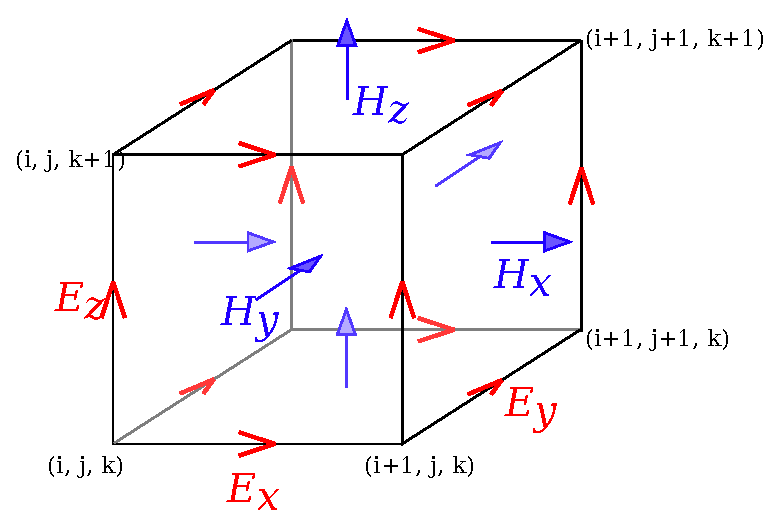
\includegraphics[width=\textwidth]{../Magisterij/Slike/Yee-cube}}
 \subfigure{
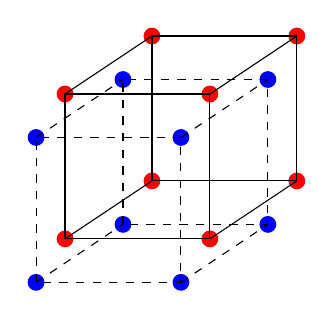
\begin{tikzpicture}[scale=.92]
    
    \foreach \x in {0,1}{
      \foreach \y in {0,1}{
        \node[mpoint] at (2*\x,2*\y) {}; 
        \node[mpoint] at (2*\x+1.2,2*\y+0.8) {}; 
        \node[epoint] at (2*\x+1.6,2*\y+1.4) {};
        \node[epoint] at (2*\x+1.6-1.2,2*\y+1.4-0.8) {};
        \draw[mgrid] (2*\x,2*\y) -- (2*\x+1.2,2*\y+0.8);
        \draw[egrid] (2*\x+1.6,2*\y+1.4) -- (2*\x+1.6-1.2,2*\y+1.4-0.8);
      }
    }
    
    \draw[mgrid] (0,0) rectangle (2,2);
    \draw[mgrid] (1.2,0.8) rectangle (3.2,2.8);
    \draw[egrid] (1.6,1.4) rectangle (3.6,3.4);
    \draw[egrid] (1.6-1.2,1.4-0.8) rectangle (3.6-1.2,3.4-0.8);
\end{tikzpicture}}
\end{figure}

\end{block}
    
  \end{column}
\end{columns}

\end{frame}

\begin{frame}{Methods -- Testing}

\begin{block}{}
\begin{columns}
  \begin{column}{.4\textwidth}

  \begin{itemize}
    \item Uniform director
    \item Refraction on interface
    \item Photonic bandgap of periodic structure
  \end{itemize}
    
  \end{column}

\begin{column}{.5\textwidth}
  \scalebox{0.4}{\input{g_test_periodic}}
\end{column}

\end{columns}


  \vspace{-25pt}
  \begin{figure}[h]
   \centering
    \subfigure{\includegraphics[width=.45\textwidth]{uniform_p}}
   \subfigure{\includegraphics[width=.4\textwidth]{refraction_p}}
  \end{figure}
  \vspace{-15pt}
\end{block}
\end{frame}

\begin{frame}{Radial-director waveguide}
\begin{block}{}
  \vspace{-20pt}
  \begin{figure}[h]
\centering
\subfigure{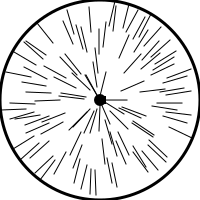
\includegraphics[height=.2\textwidth]{radial-cross}}
\subfigure{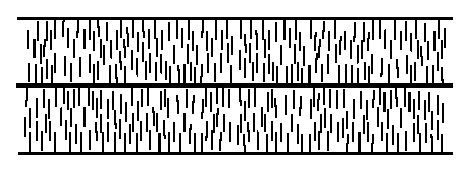
\includegraphics[height=.2\textwidth]{../Magisterij/Slike/director-profile-radial}}
\end{figure}
\end{block}

\begin{block}{}
\begin{itemize}
  \item Fibre radius 10 $\mu$m
  \item Gaussian pulse, wavelength 480 nm
  \item 8CB with $n_o = 1.51$ and $n_e = 1.68$, surrounded by water
  \item Long waveguide simulated with periodic boundary conditions
\end{itemize}
\end{block}

\end{frame}
  
\begin{frame}{Results -- Electric field}

\begin{block}{}
  \begin{itemize}
   \item Gaussian beam $\rightarrow$ Laguerre-Gaussian, dark spot at the axis
   \item The difference in refraction index deforms the beam
   \vspace{.86ex}
\end{itemize}
\end{block}

\begin{figure}[h]
\centering
 \includegraphics[width=\textwidth,clip,trim=0mm 50mm 0mm 80mm]{./render_t}
\end{figure}

\end{frame}


\begin{frame}{Results -- Pulse shape}

 \begin{figure}[h]
  \centering
  \includegraphics[width=\textwidth]{./intensity_gauss_t}
 \end{figure}

\vspace{-15pt}

\begin{block}{}
  \begin{itemize}
    \item 8 intensity regions in 2 ranks
    \item Positioned diagonally to incident polarization
    \item Two propagation modes with different polarizations
  \end{itemize}
\end{block}
\end{frame}

\begin{frame}{Results -- Propagation modes}

\begin{block}{}
\begin{columns}
  \begin{column}{.45\textwidth}
  \begin{figure}[h]
    \centering
    \includegraphics[width=.8\textwidth,clip,trim=0mm 20mm 0mm 20mm]{mode_0}
    \caption{Mode 1}
  \end{figure}  
\end{column}


\begin{column}{.45\textwidth}
  \begin{figure}[h]
    \centering
    \includegraphics[width=.8\textwidth,clip,trim=0mm 20mm 0mm 20mm]{mode_1}
    \caption{Mode 2}
  \end{figure}
    \end{column}
\end{columns}
  \vspace{-15pt}

\end{block}

\begin{block}{}
\begin{columns}
  \begin{column}{.7\textwidth}
\begin{itemize}
  \item Polarization forms -1 disclination line
  \item Disclination lines are rotated by 45$^\circ$ with respect to each other
\end{itemize}
  \end{column}

\begin{column}{.15\textwidth}
  \includegraphics[width=\textwidth]{disclination2}
\end{column}

\end{columns}

\end{block}

\end{frame}

\begin{frame}{Conclusions}
\begin{block}{Method}
 \begin{itemize}
  \item Model the propagation of light through media with non-uniform fully-anisotropic dielectric tensor
  \item Direct solving of discretized Maxwell's equations
 \end{itemize}
\end{block}
\begin{block}{Results}
 \begin{itemize}
  \item Topological defect in LC $\rightarrow$ topological defect in optical field
  \item Propagation modes of a radial-director liquid crystal waveguide
  \item Splitting of a single pulse into eight intensity regions
 \end{itemize}
\end{block}
\end{frame}

\end{document}
